\documentclass[12pt,a4paper]{article}

% 如果需要中文支持,推荐使用xeCJK + 字体设置
\usepackage{xeCJK}
\setCJKmainfont{SimSun}  % 示例:宋体,可根据系统字体情况更换
\usepackage{amsmath}      % 数学公式(如有需要)
\usepackage{graphicx}     % 插图
\usepackage{geometry}     % 调整页边距
\usepackage{fancyhdr}     % 自定义页眉页脚
\usepackage{indentfirst}  % 中文首行缩进
\usepackage{calc}         % 允许做长度运算(测量文字宽度等)
\usepackage{titlesec}
\usepackage{booktabs} % 解决 \midrule 和 \bottomrule 报错
\usepackage{enumitem} % 支持自定义列表格式
\usepackage{float}

% 设置 \section 级标题为:加粗、大字号(如 \Large)
\titleformat{\section}
	{\bfseries\large}    % 标题自身的格式
	{\thesection}        % 标题编号的显示方式
	{1em}                % 编号与标题文字之间的间距
	{}                   % 在标题文字前后可插入额外代码,此处为空
	
% 设置 \subsection 级标题为:加粗、中等字号(如 \normalsize)
\titleformat{\subsection}
	{\bfseries\normalsize}
	{\thesubsection}
	{1em}
{}

% 页面设置(可根据需要微调)
\geometry{
	left=2cm,
	right=2cm,
	top=1cm,
	bottom=1.5cm
}

% 不需要过大的行距,使用较接近单倍行距的设置
\renewcommand{\baselinestretch}{1}

% 仅在页脚居中显示页码,页眉保持为空
\pagestyle{fancy}
\fancyhf{}  % 清空默认的页眉页脚
\fancyfoot[C]{\thepage}
\renewcommand{\headrulewidth}{0pt}
\renewcommand{\footrulewidth}{0pt}

% 首行缩进2字符(中文习惯)
\setlength{\parindent}{0pt}
\setlength{\leftskip}{2em}

\begin{document}
	%-------------------------------------------------------
	% 1 并排两个minipage:左标题、右校徽
	%   - 0.65\textwidth + 0.35\textwidth = \textwidth
	%   - 如果校徽过大或过小,可改宽度,如 0.25\textwidth、0.3\textwidth 等
	%   - 如果想让标题更大,可将 \Huge 改成 \huge 或 \LARGE
	%-------------------------------------------------------
	\noindent
	\hspace{-2em}
	\begin{minipage}[c]{0.65\textwidth}
		\raggedright
		{\fontsize{40pt}{60pt}\selectfont 物理实验报告}
	\end{minipage}
	\begin{minipage}[c]{0.35\textwidth}
		\raggedleft
		% 强制把校徽拉大到 0.35\textwidth 宽度 (高度自动匹配)
		% 若想指定高度,可用 "height=3cm" 等. 二选一即可.
		
\includegraphics[width=\linewidth, trim={20cm 20cm 20cm 20cm}, clip]{university_logo.png}
	\end{minipage}

	\vspace{-1em}
	

	%下方画两条分割线,并在两线之间写学号、姓名、日期、时间
	
	\hrule
	\vspace{0.4em}
	\noindent
	\begin{tabular}{l l l l}
    学号:\underline{114514} & 姓名:\underline{SUSTech} &
    日期:\underline{2025/03/11} & 时间:\underline{周二下午}
	\end{tabular}
	\vspace{-0em}
	\par
	\hrule

	

	%正文示例

	
	\section{实验名称:光电效应法测普朗克常量}

	\section{实验目的}
	了解光电效应的基本规律,用光电效应方法测量普朗克常量\textit{h}、材料的逸出功\textit{A}和红限值$\textit{v}_{0}$
	
	\section{实验仪器}
	光电管、滤波片、汞灯、微电流计、直流电源、直流电压计等
	
	\section{实验原理}
	光电效应是指光照射在物体上,使电子获得能量并逸出物体表面的现象,逸出的电子称为光电子。这一现象表明光具有粒子性,对认识光的本性具有重要意义。\\
	光电效应实验原理如图 7.2-1 所示,其中 S 为真空光电管。当无光照射阴极时,电路中无电流流过;当短波单色光照射阴极 K 时,会产生光电流,其大小随加速电势差 $U$ 变化,形成特定的伏安特性曲线。
	\begin{figure}[htbp]
		\centering
		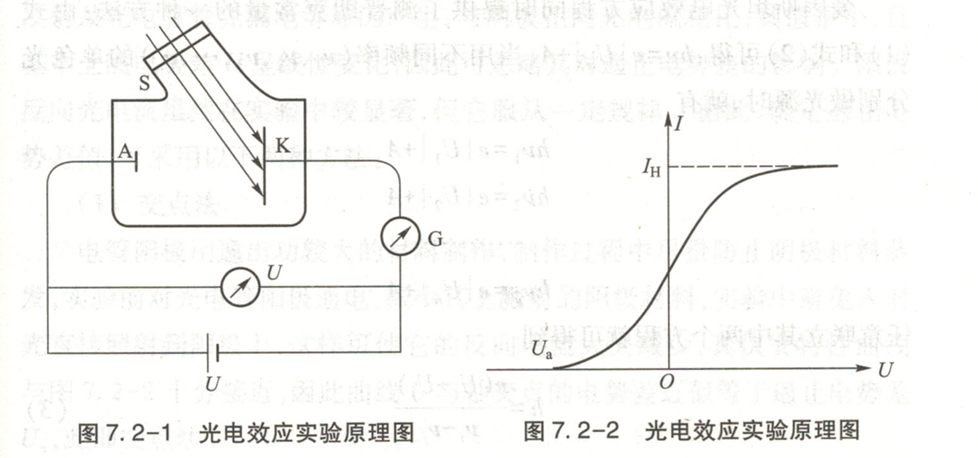
\includegraphics[width=0.5\textwidth]{实验原理图1.png}
		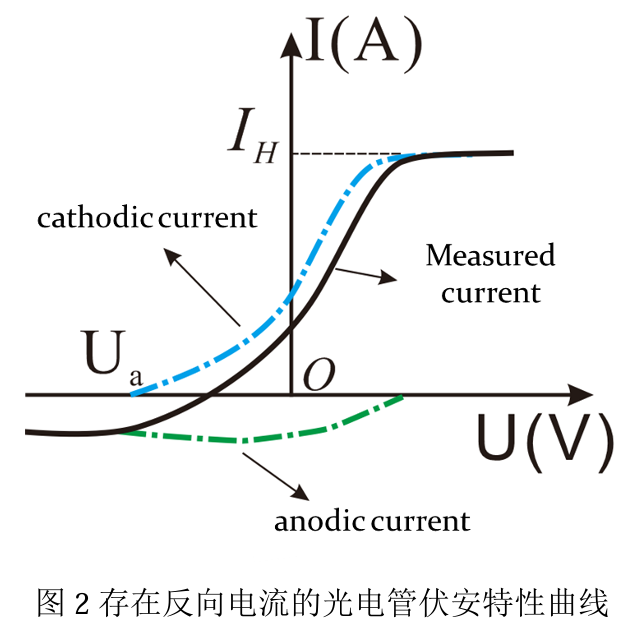
\includegraphics[width=0.2\textwidth]{光电管伏安特性曲线.png}
		\caption{光电效应实验原理图}
		\label{fig:chart1}
	\end{figure}

	\subsection{光电流与入射光强度的关系}
	光电流随加速电势差 \( U \) 增大而增加,并在饱和值 \( I_h \) 处趋于稳定,其大小与光强成正比而与频率无关。当 \( U \) 为负值时,光电流迅速减小,达到遏止电势差时降为零。

	\subsection{光电子的初动能与入射光频率之间的关系}

	根据爱因斯坦提出的光子假设,光子能量为 $\varepsilon = h\nu$,光电子吸收光子能量后,部分消耗用于克服逸出功 $A$,剩余部分转化为动能,遵循能量守恒公式
	\begin{equation}
	h\nu = \frac{1}{2}mv^2 + A
	\end{equation}
	即爱因斯坦光电效应方程。由此可知,光电子初动能与入射光频率 $\nu$ 呈线性关系,而与入射光强度无关。
	
	\subsection{光电效应有光电阈存在}

	实验指出,当光的频率 $\nu < \nu_0$ 时,不论用多强的光照射到物质都不会产生光电效应。根据公式$\frac{1}{2}mv^2 = eU_A$,红限频率为:\quad $\nu_0 = \frac{A}{h} \quad \text{$A$ 为逸出功,$h$ 为普朗克常量}$

		

	\subsection{测量普朗克常量的方法}

	由式(1)及初动能与电势差的关系联立可得,当不同频率 $(\nu_1, \nu_2, \dots, \nu_n)$ 的单色光照射时,满足爱因斯坦光电效应方程,为:  
	\begin{equation}
	h\nu_i = e|U_i| + A \quad (i = 1,2,\dots,n)
	\end{equation}   

	由任意两式联立可得普朗克常量及$U_{a}-\nu$关系:
	\begin{equation}
	h = \frac{e(U_i - U_j)}{\nu_i - \nu_j}\Rightarrow U_{a}=\frac{h}{e}v-\frac{A}{e}
	\end{equation}
	由此,可通过测定不同频率的单色光对应的遏止电势差或通过 $U_{a}-\nu$ 直线的斜率求出普朗克常量。
	因此,用光电效应方法测量普朗克常量的关键在于获得单色光、测得光电管的伏安特性曲线和确定遏止电势差值。\\
	但是实际实验环境并不理想,真空型光电管由于存在阳极光电效应所引起的反向电流和暗电流,所以测得的电流值偏小,即实际操作中遏制电压对应实际电流一定小于0(如Figure 1.图2),故我们选择拐点数据点作为特征点进行线性回归分析。

	\section{实验内容}
	\subsection{测定光电管的伏安特性曲线 ( \(-2V \sim 0V\))}
	
	以Figure 2方式接线,分别在波长为 577nm、546nm、436nm、405nm、365nm 五种单色光下测量光电管的伏安特性曲线。要求在每种单色光下,将外加电压调整至 \(-2V \sim 0V\) 范围内,每隔 0.1V 记录一个数据点,根据所得曲线确定对应的遏止电势差值。

	\begin{figure}[htbp]
		\centering
		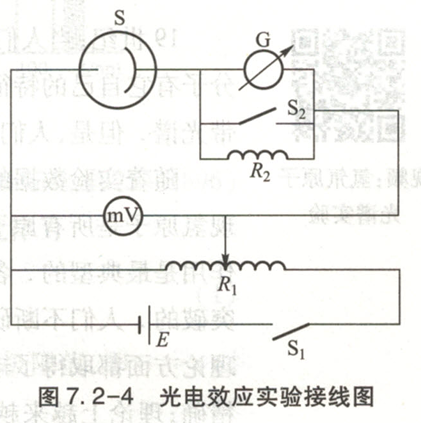
\includegraphics[width=0.3\textwidth]{接线图.png}
		\caption{实验图接线图}
		\label{fig:chart1}
	\end{figure}

	\subsection{作$U_a-\nu$ 的关系曲线,用一元线性回归法计算光电管阴极材料的红限频率$\nu_0$、逸出功$A$及普朗克常量$h$,并与公认值比较(公认值$h=6.626\times$$10^{-34}$J$\cdot$s)}

	\section{数据记录}
	按实验规范,记录数据及整理
	\begin{figure}[H]
		\centering
		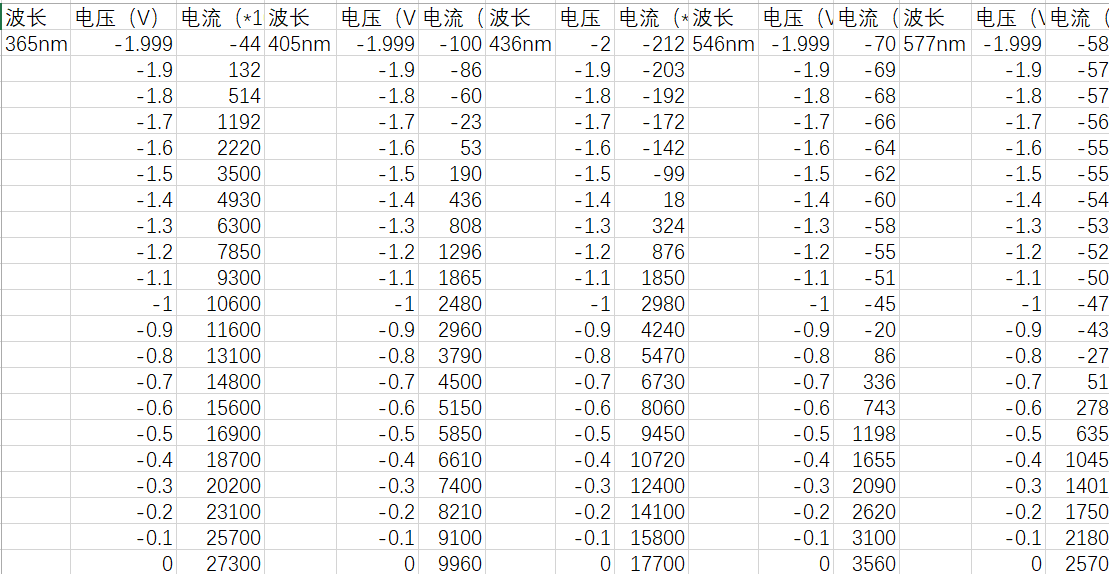
\includegraphics[width=0.6\textwidth]{实验数据汇总.png}
		\caption{原始数据整理}
		\label{fig:chart1}
	\end{figure}

	\section{数据处理}

	\subsection{不同波长单色光下光电管的伏安特性曲线}
	根据实验原始数据,绘制不同波长单色光下光电管的伏安特性曲线\\
	\begin{figure}[H]
		\centering
		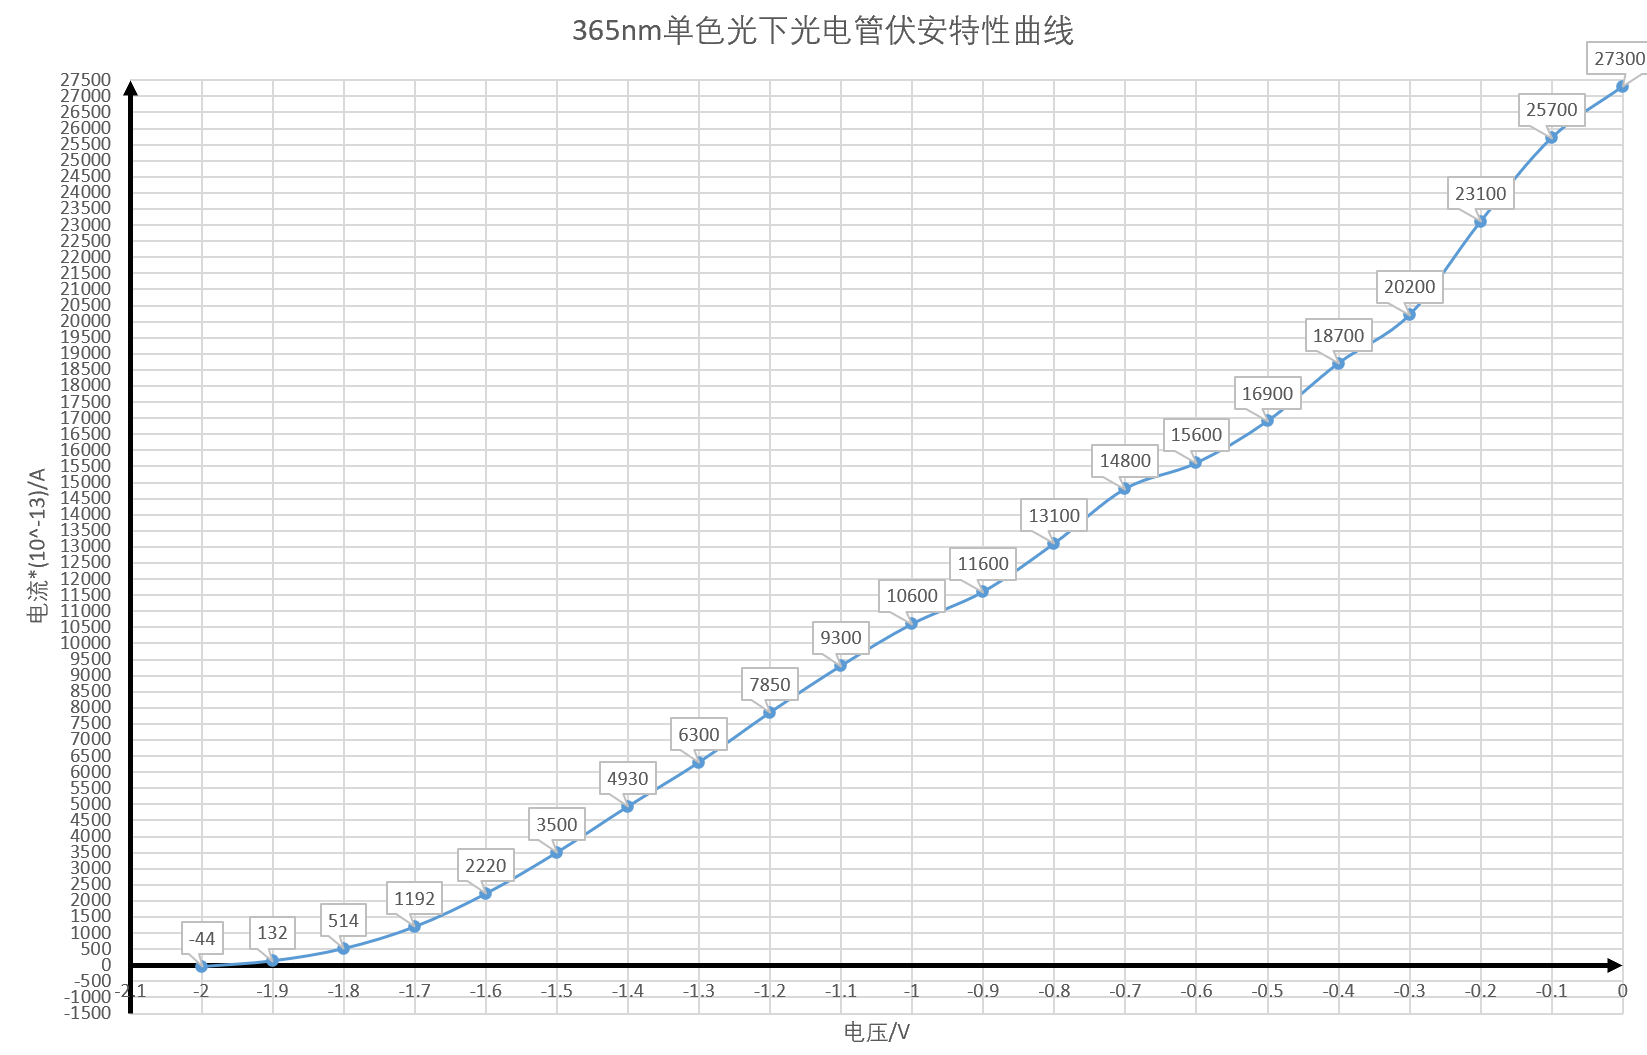
\includegraphics[width=0.49\textwidth]{365nm.png}
		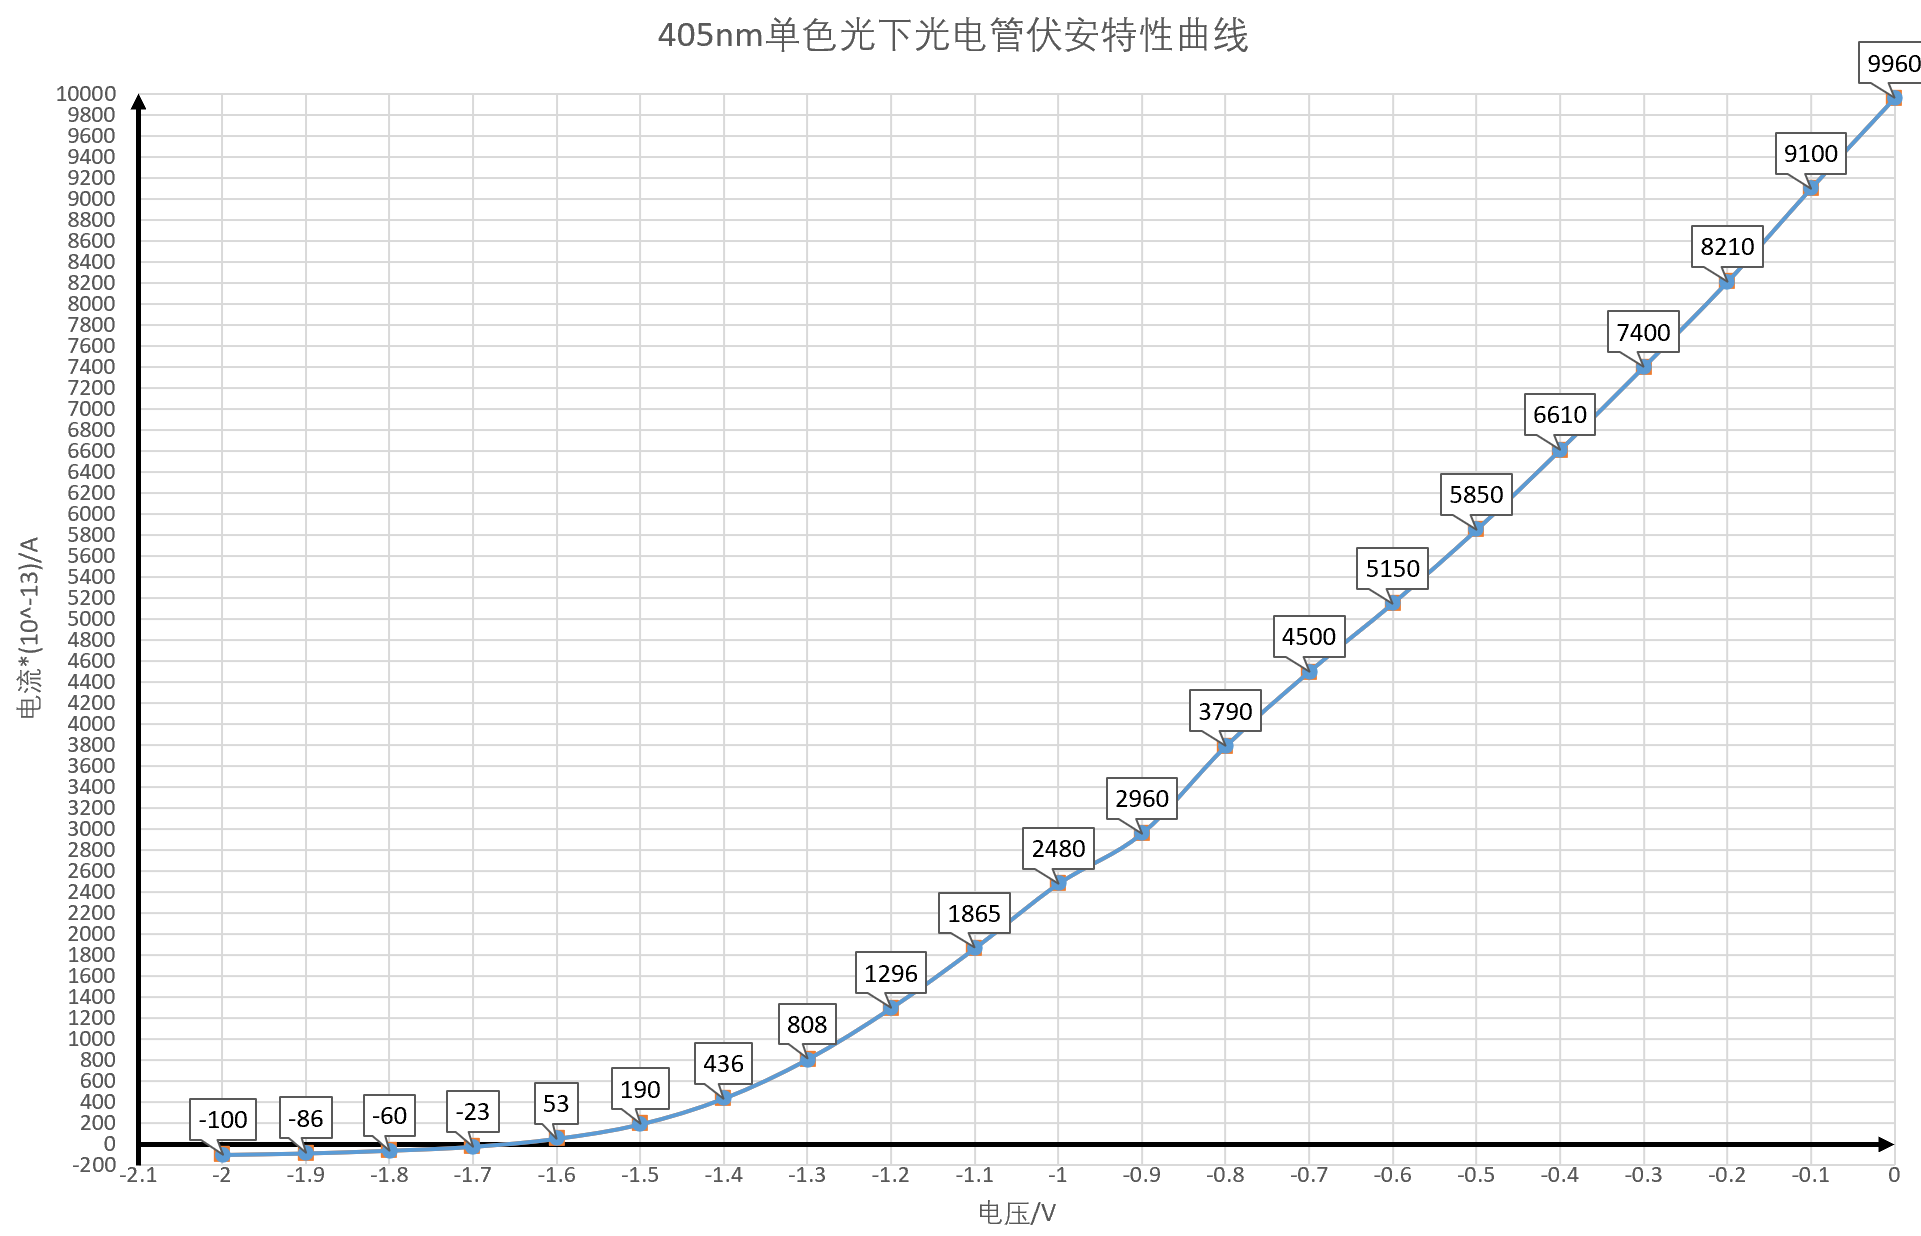
\includegraphics[width=0.49\textwidth]{405nm.png}
		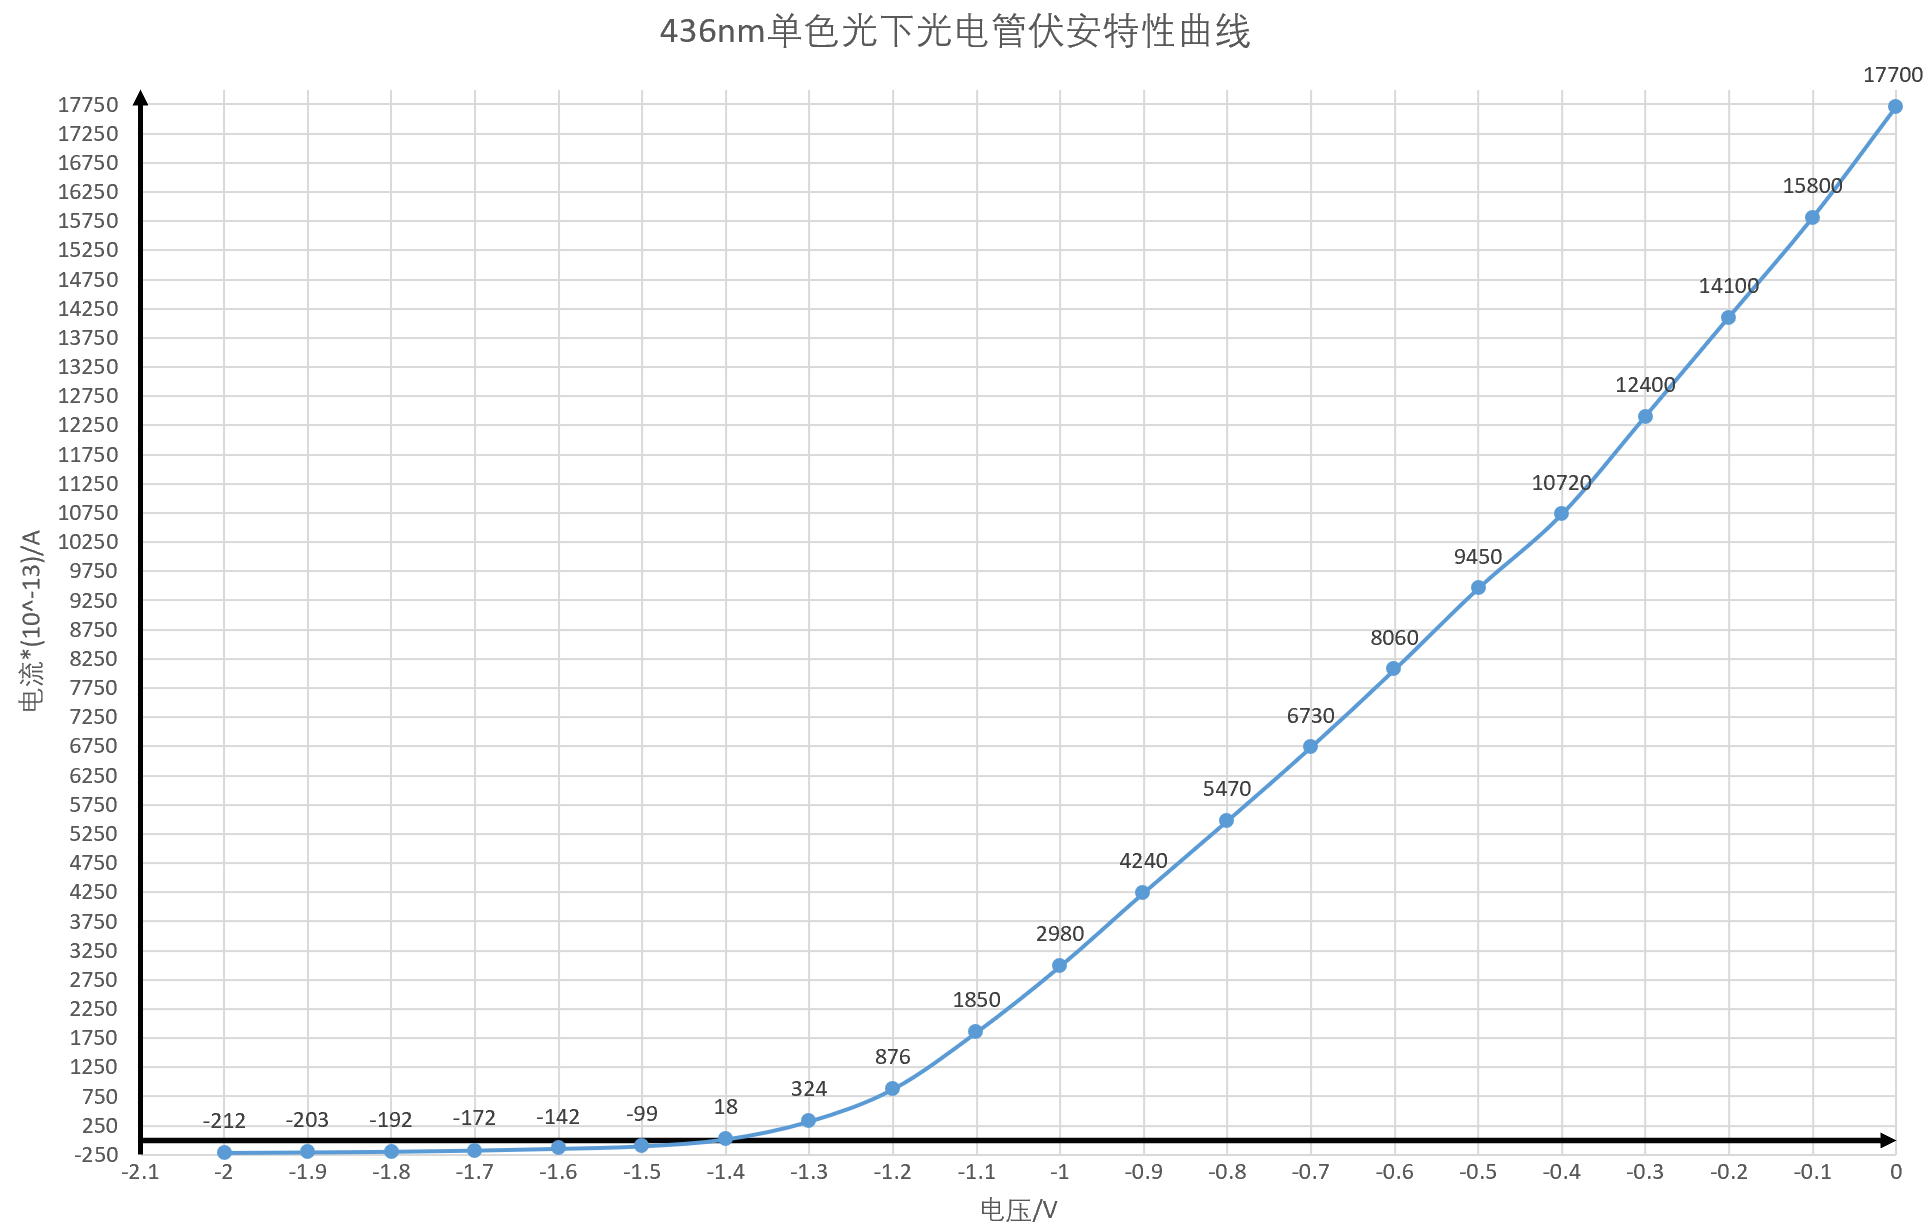
\includegraphics[width=0.49\textwidth]{436nm.png}
		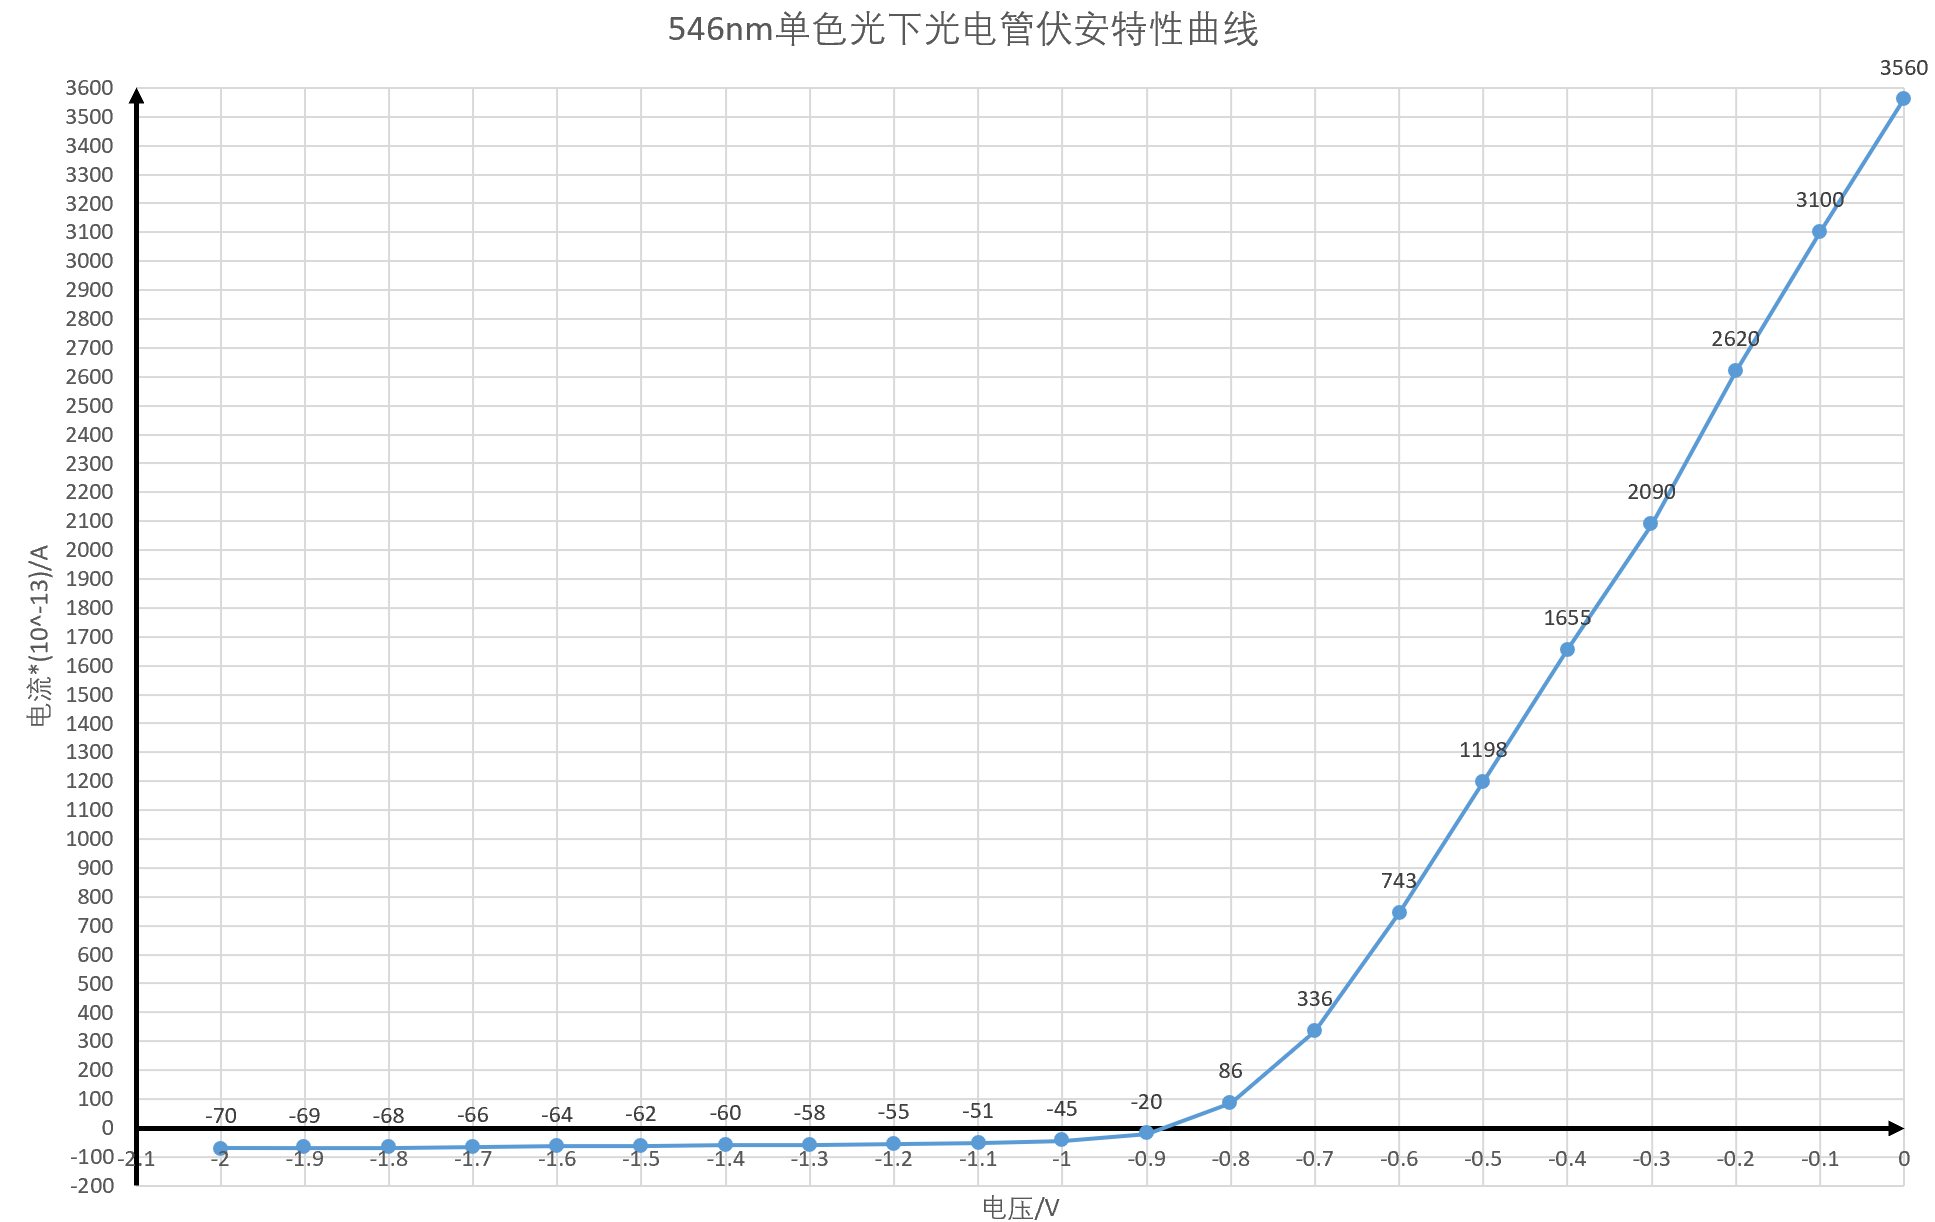
\includegraphics[width=0.49\textwidth]{546nm.png}
		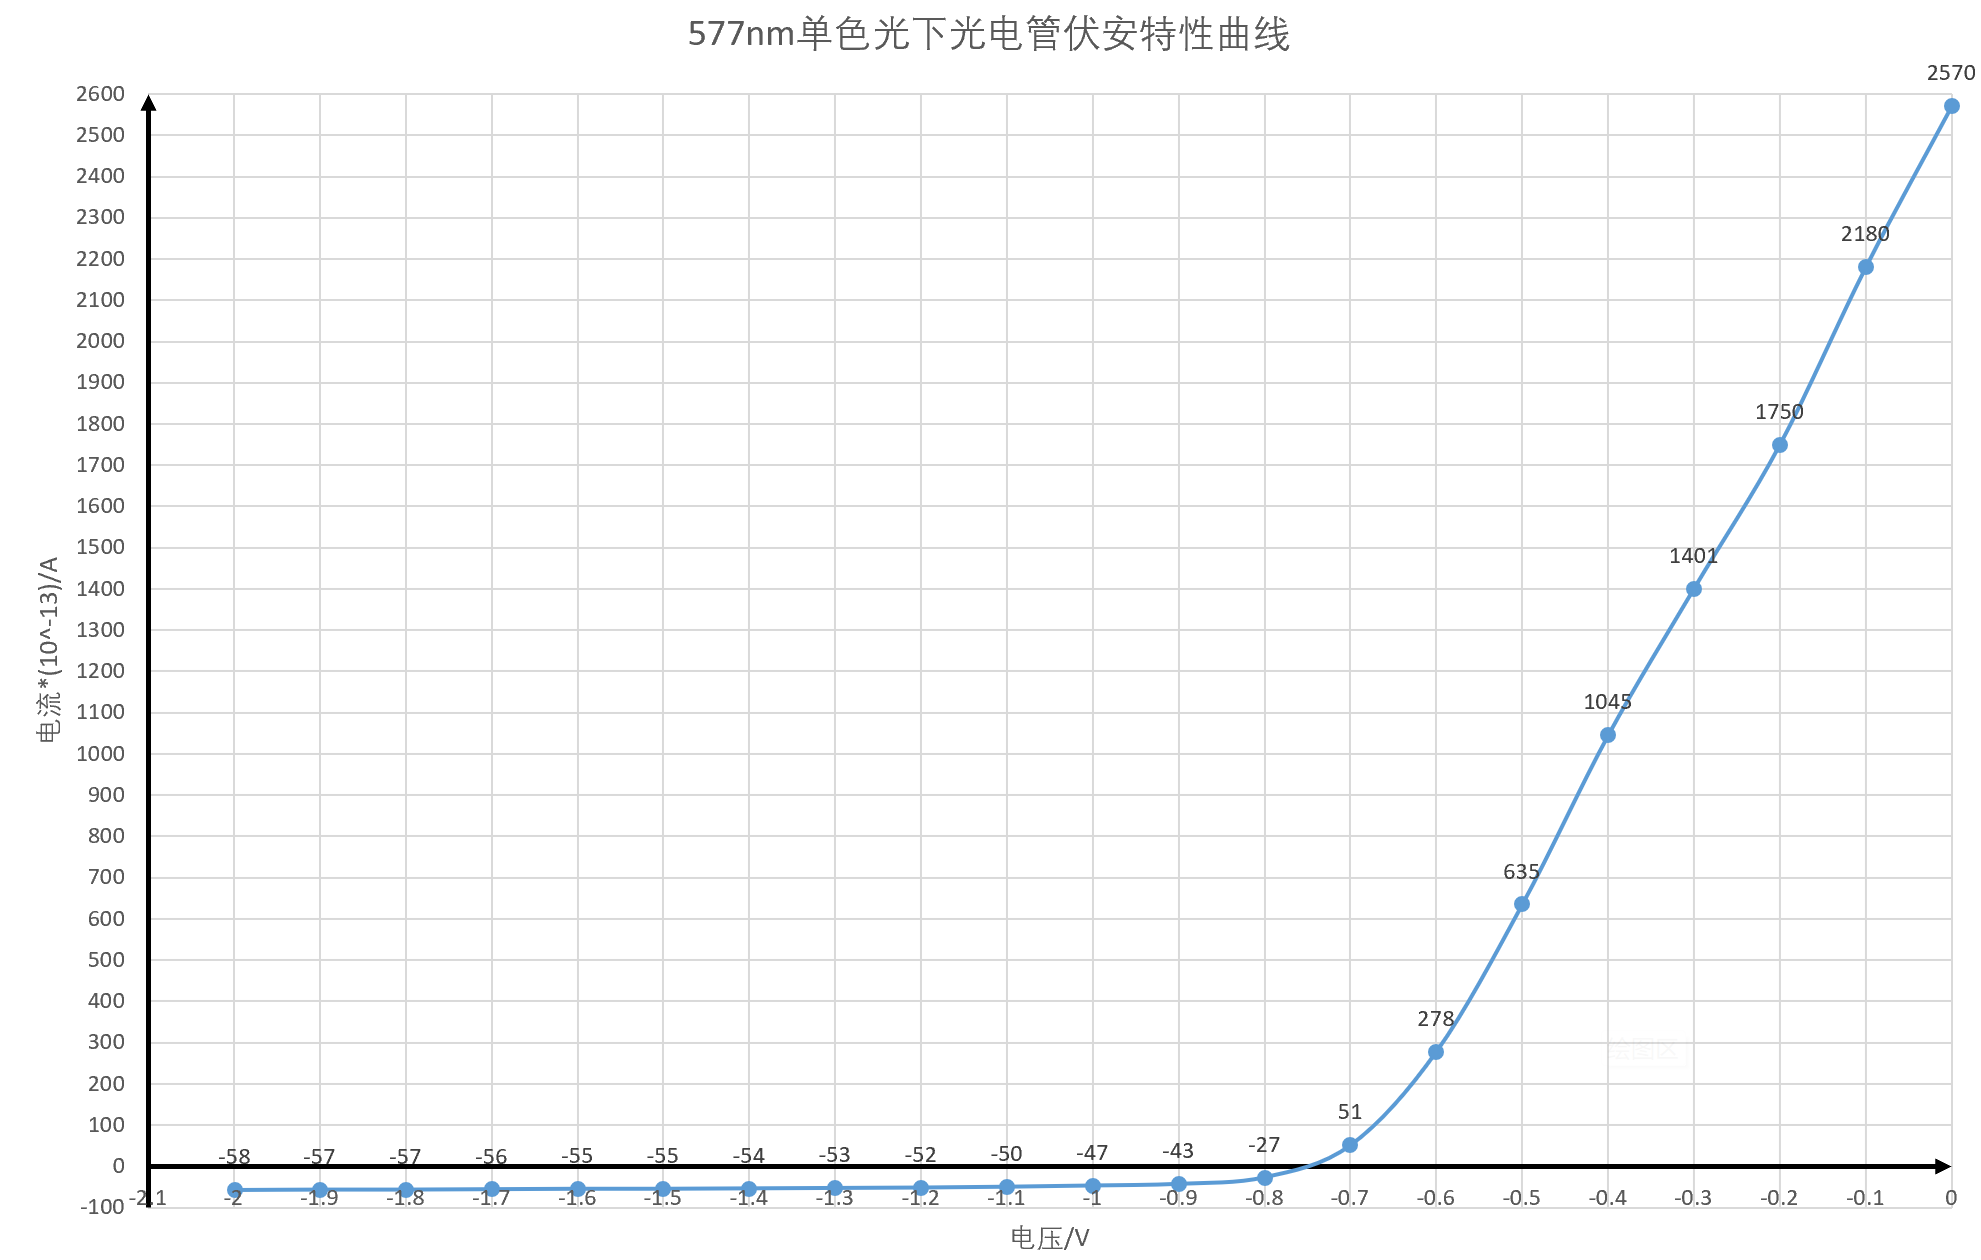
\includegraphics[width=0.49\textwidth]{577nm.png}
		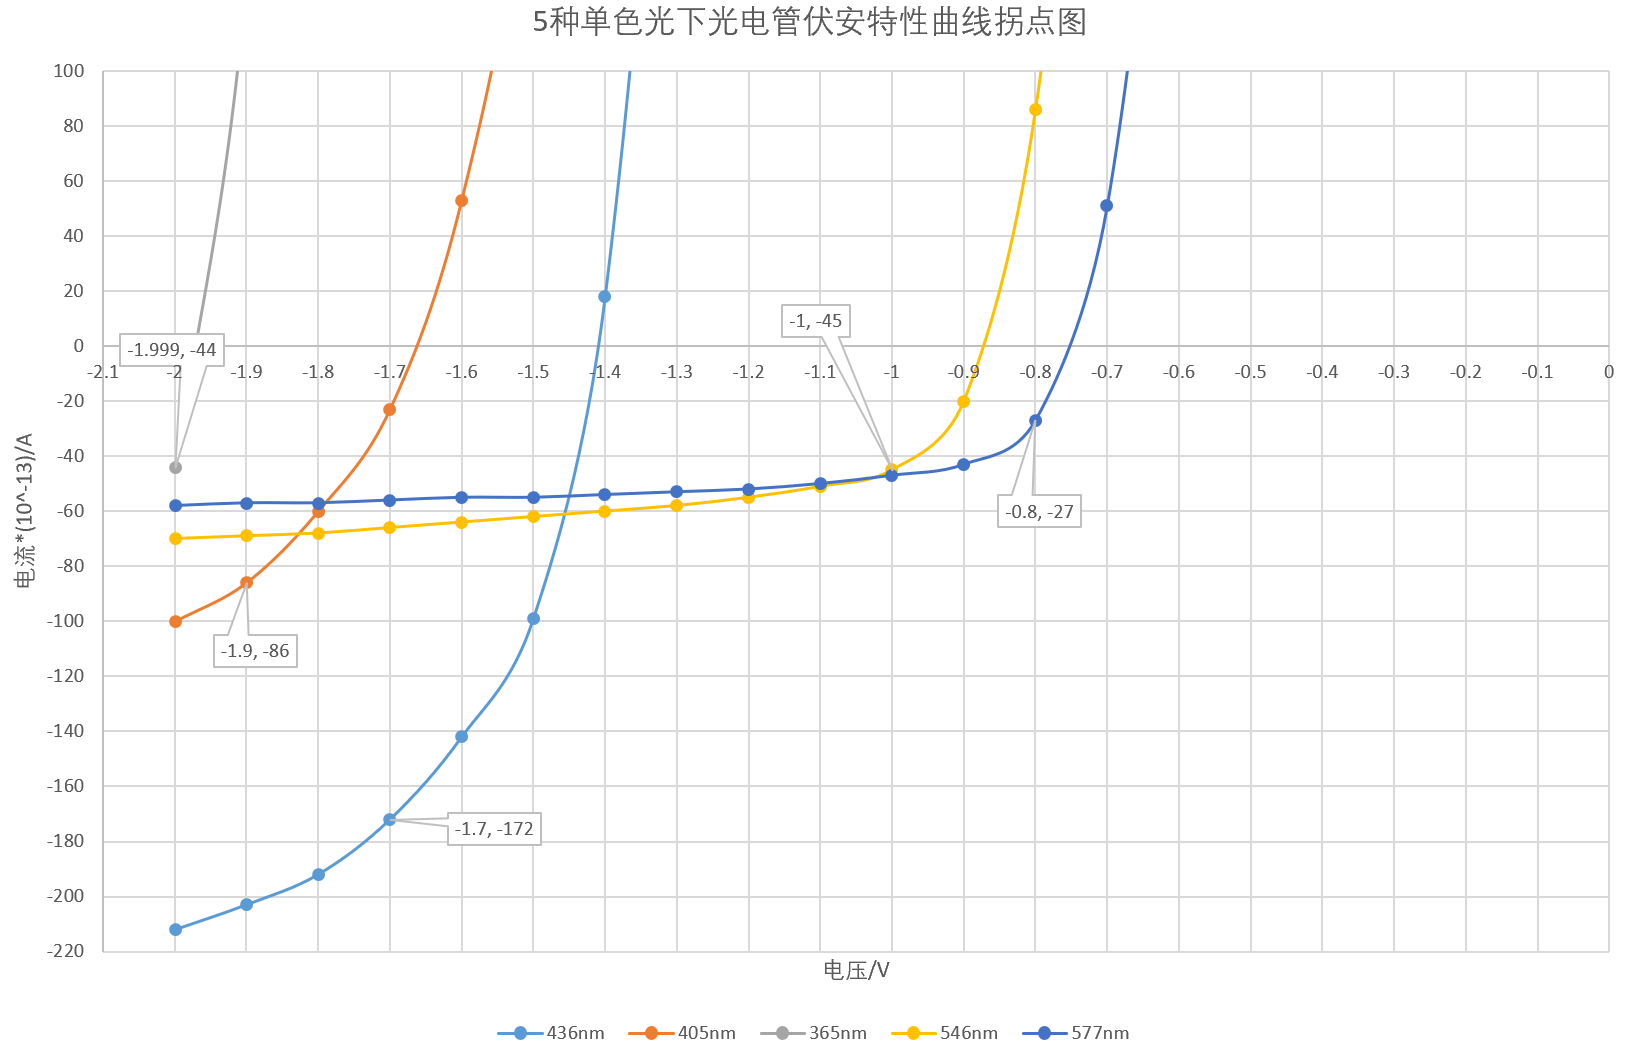
\includegraphics[width=0.49\textwidth]{拐点图.png}
		\caption{5种单色光下光电管伏安特性曲线}
		\label{fig:chart1}
	\end{figure}

	\subsection{5种单色光的遏止电压}
	由\quad Figure 4:5种单色光下光电管伏安特性曲线拐点图\quad 可得出5种单色光的遏止电压(取绝对值),如下图:
	\begin{figure}[htbp]
		\centering
		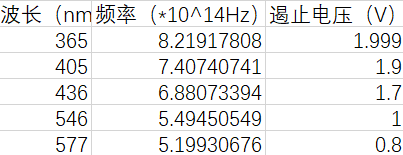
\includegraphics[width=0.75\textwidth]{遏止电压.png}
		\caption{5种单色光的遏止电压}
		\label{fig:chart1}
	\end{figure}

	\subsection{基于实验数据的线性回归拟合}
	基于上述实验数据的处理结果及 $U_{a} - \nu$ 关系公式:
	\begin{equation}
	U_{a} = \frac{h}{e} \nu - \frac{A}{e}
	\end{equation}
	拟合得到的线性回归方程如下图所示:
	
	\begin{figure}[htbp]
		\centering
		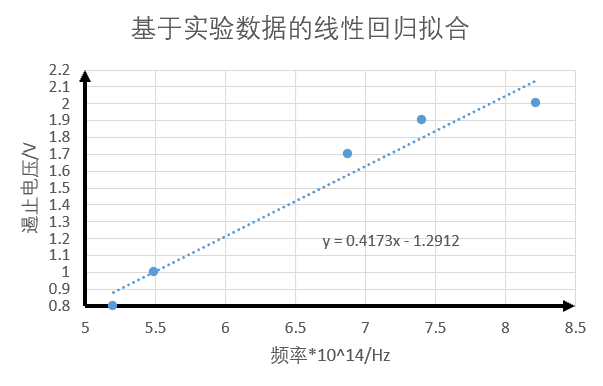
\includegraphics[width=0.75\textwidth]{拟合.png}
		\caption{$U_{a} - \nu$ 关系图}
		\label{fig:Ua-nu}
	\end{figure}

	\subsection{基于线性回归计算光电管阴极材料的红限值$\nu_0$}
	红限值对应的是遏止电压 $U = 0$,此时光电子刚好被阻止释放。根据拟合表达式:
	\[
	U = 0.4173\nu - 1.2912
	\]
	令 $U = 0$,解得:
	\[
	\nu_0 = 3.093 \times 10^{14} Hz
	\]
	因此,红限频率$\nu_0$为:
	\[
	\nu_{\text{threshold}} = 3.093 \times 10^{14} \, \text{Hz}
	\]

	\subsection{基于线性回归计算光电管阴极材料的逸出功$A$}
	逸出功$A$对应的是频率$\nu_0$=0。根据拟合表达式$U = 0.4173\nu - 1.2912$及逸出功$A$计算公式$ A = e \cdot (-b)$,
	代入已知 $b = -1.2912 \, \text{V}$,以及 $e = 1.602 \times 10^{-19} \, \text{C}$:
	\[
	A = 1.602 \times 10^{-19} \cdot 1.2912
	  = 2.068 \times 10^{-19} \, \text{J}
	\]
	因此,逸出功$A$为:
	\[
		A = 2.068 \times 10^{-19} \, \text{J}
	\]

	\subsection{基于线性回归计算普朗克常数$h$}
	由斜率 $k = \frac{h}{e} = 0.4173 \, \text{(V·s)}$ 可得,
	$$h = k \cdot e$$
	其中,$e$ 为电子电荷,取 $e = 1.602 \times 10^{-19} \, \text{C}$,代入计算:
	\[
	h = 0.4173 \times 10^{-14} \cdot 1.602 \times 10^{-19}
	  = 6.686 \times 10^{-34} \, \text{J·s}
	\]
	由此计算得普朗克常数为:
	$$h \approx 6.686 \times 10^{-34} \, \text{J·s}$$
	由此可以看出,实验结果与标准普朗克常数 $h_{\text{standard}} = 6.626 \times 10^{-34} \, \text{J·s}$ 非常接近,验证了实验的准确性。

	\section{误差分析}
	由百分比误差公式计算可得:
	\[
	\frac{\Delta h}{h} = \frac{|h_{\text{实际}} - h|}{h} \times 100\% = \frac{|6.626 \times 10^{-34} - 6.686 \times 10^{-34}|}{6.626 \times 10^{-34}} \times 100\%
	\]
	\[
	\frac{\Delta h}{h} = \frac{0.06 \times 10^{-34}}{6.626 \times 10^{-34}} \times 100\% \approx 0.906\%<1\%
	\]
	随机误差(Random Error)\\
	电流不稳定 致读数误差:由于电流波动引起的不规则变化,导致测量值随机波动。\\
	单色光强度的随机波动:高压汞灯本身可能会因为供电电压的微小变化或环境因素导致光强的不规则波动,进而影响实验结果。\\
	系统误差(Systematic Error)\\
	实验环境中由于遮挡环境光有限,使得单色光不稳定:外界环境光的遮挡不足造成单色光不稳定,是一种固定偏差。\\
	读取光电流的仪器精确度档位之间存在一定分断误差,换档后精度发生改变:仪器设计上的固有误差,导致测量精度因档位不同而变化。\\
	长时间实验,光电管温度会显著升高,存在热激发电子干扰:温度升高的系统性变化,会逐步影响实验结果。\\
	人为误差(Human Error)\\
	拐点的选取存在主观因素,可能存在较大误差:拐点选择依赖实验者的主观判断,可能引入明显误差。
	
	\section{实验结论}
	本实验通过光电效应,利用拐点法、线性回归等方法,求得了普朗克常量\textit{h}、材料的逸出功\textit{A}和红限值$\textit{v}_{0}$
	$$h \approx 6.686 \times 10^{-34} \, \text{J·s} \quad \quad \text{(误差百分比约为0.906\%)}$$
	\[
		A = 2.068 \times 10^{-19} \, \text{J}
	\]
	\[
	\nu_0 = 3.093 \times 10^{14} Hz
	\]


\end{document}
